

\tikzset{every picture/.style={line width=0.75pt}} %set default line width to 0.75pt        

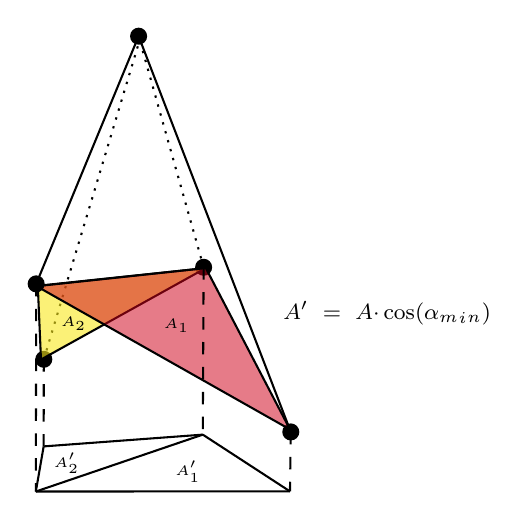
\begin{tikzpicture}[x=0.75pt,y=0.75pt,yscale=-1,xscale=1]
%uncomment if require: \path (0,300); %set diagram left start at 0, and has height of 300

%Shape: Circle [id:dp20203675621890882] 
\draw  [fill={rgb, 255:red, 0; green, 0; blue, 0 }  ,fill opacity=1 ] (75,183.4) .. controls (75,181.41) and (76.61,179.8) .. (78.6,179.8) .. controls (80.59,179.8) and (82.2,181.41) .. (82.2,183.4) .. controls (82.2,185.39) and (80.59,187) .. (78.6,187) .. controls (76.61,187) and (75,185.39) .. (75,183.4) -- cycle ;
%Shape: Circle [id:dp4460917567211786] 
\draw  [fill={rgb, 255:red, 0; green, 0; blue, 0 }  ,fill opacity=1 ] (152,139.07) .. controls (152,137.08) and (153.61,135.47) .. (155.6,135.47) .. controls (157.59,135.47) and (159.2,137.08) .. (159.2,139.07) .. controls (159.2,141.05) and (157.59,142.67) .. (155.6,142.67) .. controls (153.61,142.67) and (152,141.05) .. (152,139.07) -- cycle ;
%Shape: Circle [id:dp23372343609699975] 
\draw  [fill={rgb, 255:red, 0; green, 0; blue, 0 }  ,fill opacity=1 ] (194,218.4) .. controls (194,216.41) and (195.61,214.8) .. (197.6,214.8) .. controls (199.59,214.8) and (201.2,216.41) .. (201.2,218.4) .. controls (201.2,220.39) and (199.59,222) .. (197.6,222) .. controls (195.61,222) and (194,220.39) .. (194,218.4) -- cycle ;
%Shape: Circle [id:dp7435513334633294] 
\draw  [fill={rgb, 255:red, 0; green, 0; blue, 0 }  ,fill opacity=1 ] (120.67,27.73) .. controls (120.67,25.75) and (122.28,24.13) .. (124.27,24.13) .. controls (126.25,24.13) and (127.87,25.75) .. (127.87,27.73) .. controls (127.87,29.72) and (126.25,31.33) .. (124.27,31.33) .. controls (122.28,31.33) and (120.67,29.72) .. (120.67,27.73) -- cycle ;
%Straight Lines [id:da9245497792530712] 
\draw [color={rgb, 255:red, 0; green, 0; blue, 0 }  ,draw opacity=1 ] [dash pattern={on 0.84pt off 2.51pt}]  (78.6,183.4) -- (124.27,31.33) ;
%Straight Lines [id:da7005143254135355] 
\draw [color={rgb, 255:red, 0; green, 0; blue, 0 }  ,draw opacity=1 ] [dash pattern={on 0.84pt off 2.51pt}]  (155.6,139.07) -- (124.27,27.73) ;
%Straight Lines [id:da28064823401026573] 
\draw    (197.6,218.4) -- (124.27,27.73) ;
%Shape: Triangle [id:dp11918551614132744] 
\draw  [fill={rgb, 255:red, 248; green, 231; blue, 28 }  ,fill opacity=0.6 ] (77.24,183.52) -- (156.66,139.45) -- (75.71,148) -- cycle ;
%Shape: Triangle [id:dp7709931078112477] 
\draw  [fill={rgb, 255:red, 208; green, 2; blue, 27 }  ,fill opacity=0.52 ] (197.19,217.19) -- (75.12,148.19) -- (156.66,139.45) -- cycle ;
%Straight Lines [id:da7697818424224974] 
\draw [fill={rgb, 255:red, 0; green, 0; blue, 0 }  ,fill opacity=1 ]   (74.93,147.07) -- (124.27,27.73) ;
%Shape: Circle [id:dp25664476075983755] 
\draw  [fill={rgb, 255:red, 0; green, 0; blue, 0 }  ,fill opacity=1 ] (71.33,147.07) .. controls (71.33,145.08) and (72.95,143.47) .. (74.93,143.47) .. controls (76.92,143.47) and (78.53,145.08) .. (78.53,147.07) .. controls (78.53,149.05) and (76.92,150.67) .. (74.93,150.67) .. controls (72.95,150.67) and (71.33,149.05) .. (71.33,147.07) -- cycle ;
%Straight Lines [id:da5723635368812333] 
\draw  [dash pattern={on 4.5pt off 4.5pt}]  (74.93,147.07) -- (74.76,247.11) ;
%Straight Lines [id:da9477555281674963] 
\draw  [dash pattern={on 4.5pt off 4.5pt}]  (78.6,183.4) -- (78.53,225.37) ;
%Straight Lines [id:da7265146935260219] 
\draw  [dash pattern={on 4.5pt off 4.5pt}]  (155.6,139.07) -- (155.2,219.7) ;
%Straight Lines [id:da8482223625070795] 
\draw  [dash pattern={on 4.5pt off 4.5pt}]  (197.6,218.4) -- (197.2,247.03) ;
%Straight Lines [id:da135198346268814] 
\draw    (74.76,247.11) -- (197.2,247.03) ;
%Straight Lines [id:da7899881746363868] 
\draw    (155.2,219.7) -- (197.2,247.03) ;
%Straight Lines [id:da24200805108322687] 
\draw    (74.76,247.11) -- (155.2,219.7) ;
%Straight Lines [id:da38438776639593253] 
\draw    (78.53,225.37) -- (74.76,247.11) ;
%Straight Lines [id:da27704931617334616] 
\draw    (155.2,219.7) -- (78.53,225.37) ;

% Text Node
\draw (135,162.5) node [anchor=north west][inner sep=0.75pt]  [font=\tiny] [align=left] {$\displaystyle A_{1}$};
% Text Node
\draw (140.5,231) node [anchor=north west][inner sep=0.75pt]  [font=\tiny] [align=left] {$\displaystyle A'_{1}$};
% Text Node
\draw (82,227) node [anchor=north west][inner sep=0.75pt]  [font=\tiny] [align=left] {$\displaystyle A'_{2}$};
% Text Node
\draw (85.4,161.38) node [anchor=north west][inner sep=0.75pt]  [font=\tiny] [align=left] {$\displaystyle A_{2}$};
% Text Node
\draw (192.5,154) node [anchor=north west][inner sep=0.75pt]  [font=\footnotesize] [align=left] {$\displaystyle A'\ =\ A\cdotp \cos( \alpha _{m}{}_{i}{}_{n})$};


\end{tikzpicture}
